\label{taxi-availability}
\subsubsection{Purpose}

When a taxi driver is ready for a ride, he/she shall be abòe to notify the system using his mobile phone. With the app he/she can change his status from "not in service" to "in service".

When the system receives the status update from the taxi driver, it inserts him/her in the right queue for his/her taxi zone using the information from the taxi GPS if the new status is "in service", or it removes him/her from the queue if the new status is "not in service".

After a ride, a taxi driver has to notify, using the dedicated section of the app, that the ride is over. The system shall reinsert the taxi into the right queue.
%TODO define FIFO

The queues are FIFO and when a taxi driver refuses a ride, the system moves the taxi to the bottom of the same queue.

When a taxi driver accepts a ride, the system marks the taxi as busy and removes it from the top of the queue.

\subsubsection{Scenario 1}
Ernie gets in his taxi, ready to start his working day. He takes out his phone from his pocket and after logging in he changes his status in "in service".

The system acquires the changing and retrieves the GPS position of Ernie's taxi. It analyses the data and puts the taxi in the right queue.

After thirty minutes the system has an incoming request from the Ernie's zone. The first taxi on the top of the queue is Ernie's. The system sends a notification to Ernie and waits for a reply.

Ernie receives the request and accepts the meeting. The system pops Ernie from the top of the queue and marks it as busy.

When Ernie accomplishes the ride, he notifies the system, which retrieves the new GPS position and inserts Ernie's in the queue.

\subsubsection{Response sequence}
The response sequence associated with this functionality is shown in figure~\ref{fig:taxi_availability}.
\begin{figure}
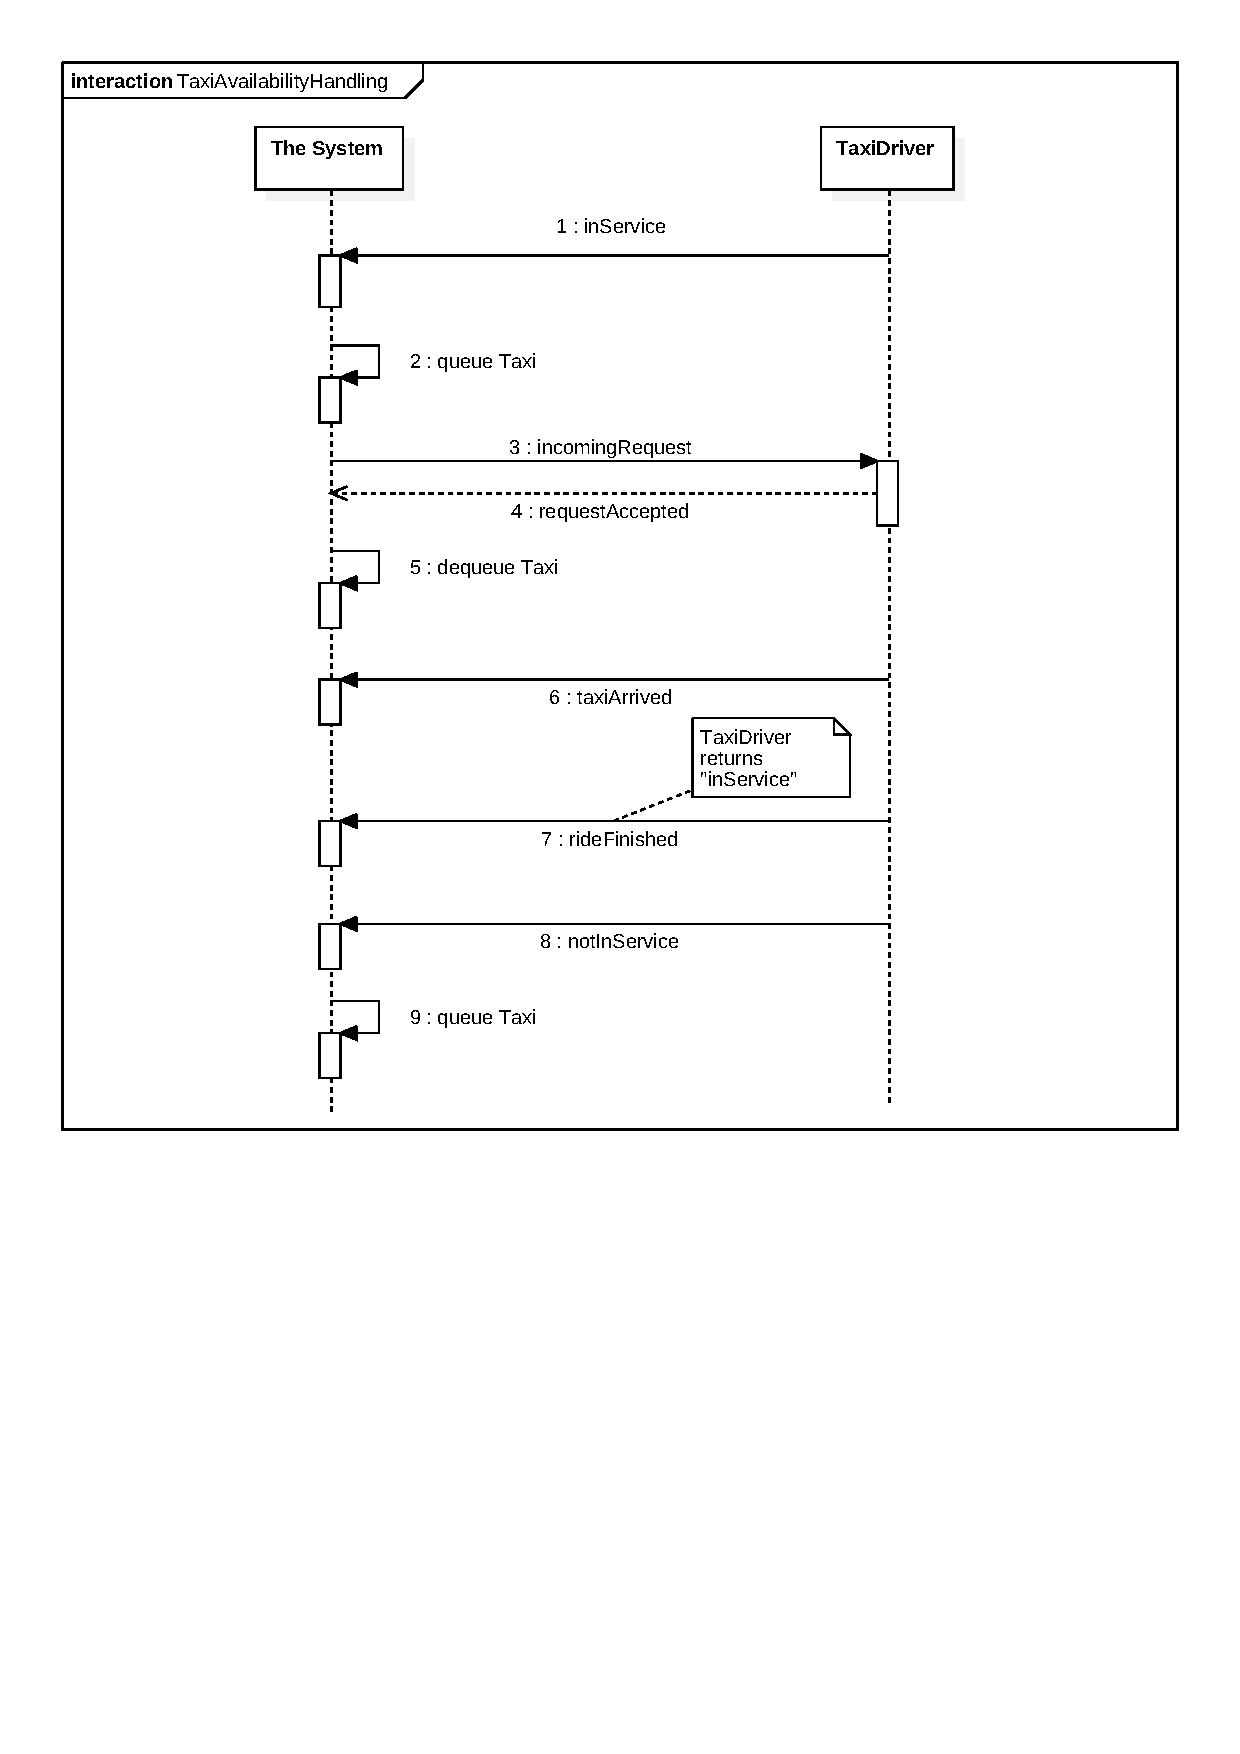
\includegraphics[width=\textwidth]{diagrams/taxi_availability_handling.pdf}
\caption{Sequence diagram of an accepted taxi call.}
\label{fig:taxi_availability}
\end{figure}

\subsubsection{Associated functional requirements}
\begin{enumerate}
\item The system knows the information about the GPS installed on the taxi.
\item The mobile app has to offer to the taxi driver the "change status" function and the "ride complete" function.
\item The system must notify the taxi when a request is incoming.
\item The system inserts the taxi in the right queue and changes it if the taxi changes area.
\item For every new request, the system chooses the taxi driver on the top of the queue.
\item The taxi driver has to reply in one minute to the request, else the ride is automatically refused.
\item The system manages the queues using the FIFO policy.
\end{enumerate}